\documentclass[a4paper,ngerman,headsepline]{scrreprt}
\KOMAoptions{fontsize=12pt}
\KOMAoptions{headings=standardclasses}
\KOMAoptions{DIV=13}
%\KOMAoption{captions}{centeredbeside}
\usepackage{scrlayer-scrpage}
\KOMAoptions{autooneside=false,automark}
\pagestyle{scrheadings}
\usepackage{scrdate,scrtime}

% LOCALISATION
\usepackage[utf8]{inputenc}
\usepackage[T1]{fontenc}
\usepackage[ngerman]{babel}
\usepackage[style=german,german=guillemets]{csquotes}
\pdfminorversion=7
\usepackage{calc}

% LAYOUT
\usepackage[activate=true,final,spacing=true,expansion=true]{microtype}

% VISUAL
\usepackage{amsmath,amssymb,amsfonts}
\usepackage{libertine}
\usepackage{inconsolata}
\usepackage{booktabs}
\usepackage{lastpage,multicol}
\usepackage{subcaption,setspace,enumerate}

% TOOLS
\usepackage[dvipsnames]{xcolor}
\usepackage{pgf,tikz}
\usepackage{siunitx}
\sisetup{locale=DE,per-mode=symbol,output-decimal-marker={,},detect-weight}

% PAGE LAYOUT
%\numberwithin{equation}{subsection}
\renewcommand*{\pagemark}{} % suppress center pagenum
\renewcommand{\thefootnote}{\roman{footnote}}
\setkomafont{pageheadfoot}{\rmfamily}
\clearpairofpagestyles
\lohead{Benutzerhandbuch \textit{htl-tk-chat}}
\rohead{Alexander Lessacher, Laurenz Preindl, Simon Graber}
\cohead{}
\rofoot{Seite \thepage\ von \pageref{LastPage}}
\cofoot{\raisebox{-2cm}{Vom \todaysname, dem \today}}

\newcommand*\diff{\mathop{}\!\mathrm{d}}

% BIBLIOGRAPHIE
%\usepackage[imakeidx]{xindex} % oldindex
\usepackage{makeidx}\makeindex
\usepackage[backend=biber,style=authoryear,natbib=true,hyperref=true]{biblatex}
\addbibresource{/home/ln/Dokumente/tex/literatur/main.bib}

\usepackage[hidelinks]{hyperref}
\usepackage{marvosym}
\hypersetup
{%
  pdfauthor={Graber, Preindl, Lessacher},%
  pdfcreator={pdfLaTeX}%
  colorlinks=true,linkcolor={black!70!blue},citecolor={blue!50!black},urlcolor={blue},%
  pdffitwindow={false},pdfstartview={FitH},%
  pdftitle={Dokumentation htl-tk-chat},pdfsubject={Software-Engineering}%
}

\begin{document}

%\subject{}
\title{Handbuch \texttt{htl-tk-chat}}
\subtitle{Projekt: Fachspezifische Softwaretechnik}
\author{Simon Graber \and Laurenz Preindl \and Alexander Lessacher}

\maketitle
\tableofcontents

\section{Einführung}
Der \texttt{htl-tk-chat} ist eine Chat-Applikation mit Qt-User-Interface. Sie können sich damit mit einem Client zu einem Server verbinden und mit den Teilnehmern dort Nachrichten austauschen. Standardmäßig geschieht dies verschlüsselt (SSL/TLS), ihre Nachrichten sind also auf dem Weg zu den anderen Teilhemern \enquote{sicher}.

\section{Start}
Es wird davon ausgegangen, dass Sie die Applikation als Client nutzen und ein bestehender Server bekannt und erreichbar ist.\\
Zum Starten des Programms rufen sie unter \texttt{frontend/client.py} auf. Hierzu können sie die Date direkt aufrufen (\texttt{./frontend/client.py} oder dem Programm \texttt{python3} als Parameter übergeben. Hierzu verwenden sie den Befehl \texttt{python3 frontend/client.py}.

\begin{figure}[ht]\centering
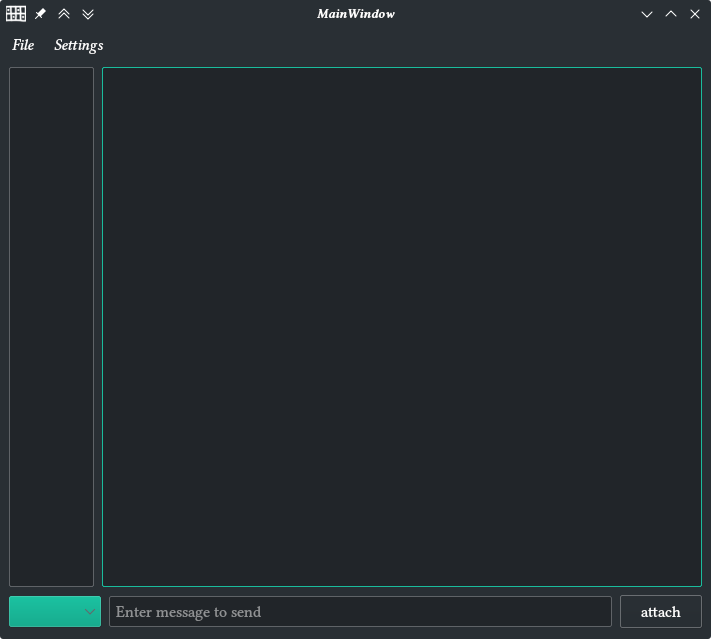
\includegraphics[width=\textwidth]{images/empty}
\caption{Nun öffnet sich das Hauptfenster des Chats}
\end{figure}

\begin{figure}[ht]\centering
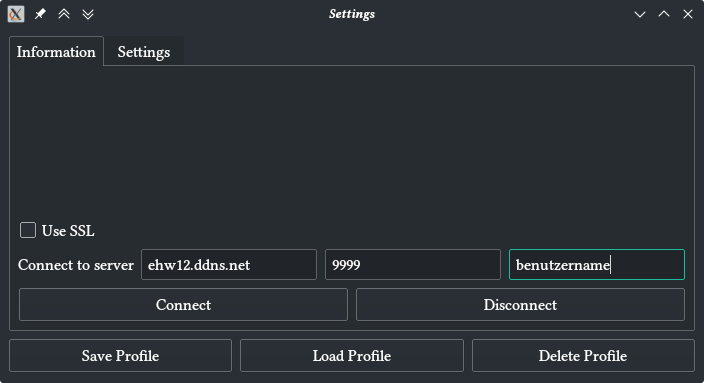
\includegraphics[width=\textwidth]{images/settings}
\caption{Zusätzlich öffnet sich das Einstellungsfenster\label{fig:settings}}
\end{figure}\clearpage
Wie in Abb. \ref{fig:settings} gezeigt, müssen Sie eine gültige Adresse eines \texttt{htl-tk-chat}-Servers in das dafür vorgesehene Feld eintragen. Verwenden Sie einen Benutzernamen Ihrer Wahl. Wenn der Server Ihrer Wahl SSL unterstützt, setzen sie die Checkbox \enquote{Use SSL}.
Speichern Sie Ihre Daten mittels drücken des Buttons \enquote{Save Profile}. Um sich zum Server zu verbinden drücken Sie \enquote{Connect}. Nun können Sie das Einstellungsfenster schließen und zum Hauptfenster zurükkehren. (Siehe Abb. \ref{fig:alone})

\begin{figure}[ht]\centering
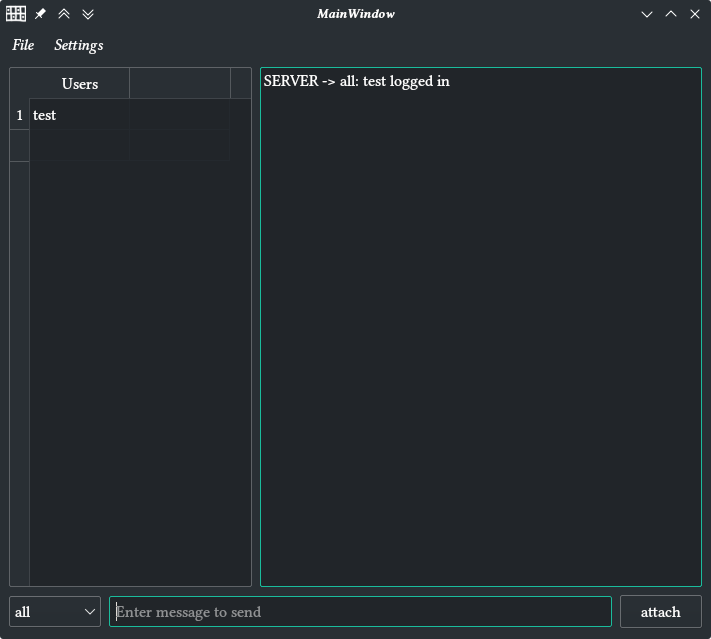
\includegraphics[width=\textwidth]{images/alone}
\caption{Der Chat-Client ist nun verbunden, Sie können nun Nachrichten empfangen und versenden \label{fig:alone}}
\end{figure}

Um Nachrichten zu verfassen, tippen Sie den Text in die Eingabezeile am unteren Rand des Fensters ein und drücken die Enter-Taste.% \LKeyEnter ging nicht ...

\begin{figure}[ht]\centering
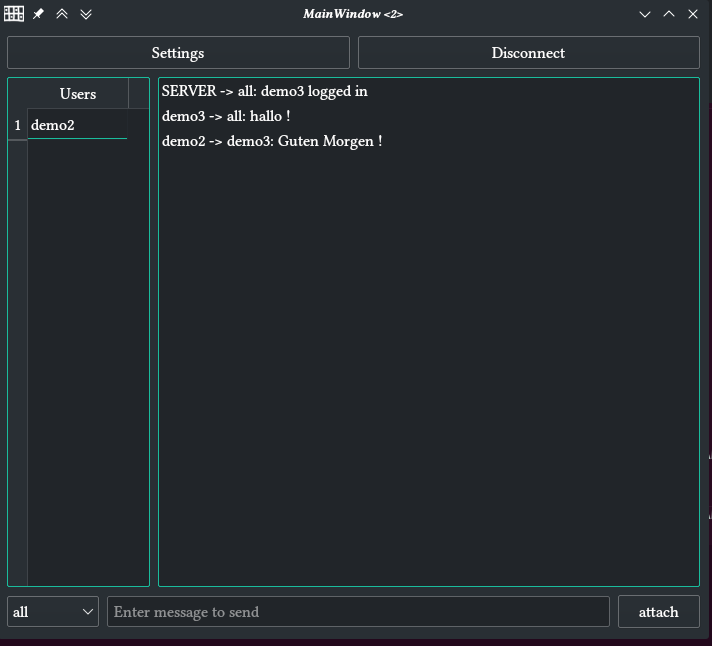
\includegraphics[width=\textwidth]{images/conversation}
\caption{Nun können Sie im DropDown-Menü in der linken unteren Ecke den Empfänger Ihrer Nachricht auswählen und mit Enter versenden. Empfangene Nachrichten werden Ihnen in der rechten Hälfte des Fensters angezeigt.\label{fig:conversation}}
\end{figure}


\begin{figure}[ht]\centering
\includegraphics[width=\textwidth]{images/attach-image}
\caption{Sie können durch drücken des \texttt{attatch}-Buttons in der rechten unteren Ecke des Fensters eine Bilddatei anhängen, es öffnet sich ein FileChooser-Dialog des Betriebssystems und Sie können dort zu dem Bild Ihrer Wahl navigieren. Haben Sie das Bild ausgewählt wird es an den gewählten Empfänger versendet.\label{fig:attach-image}}
\end{figure}

\end{document}
